
\section{Evaluation}
\label{sec:evaluation}

Our evaluation evaluates \ourtool's
effectiveness in the following our aspects:

\begin{itemize}
\item Is the supported SQL subset expressive enough to describe
a variety of queries?
\item the time cost of \ourtool in sythesizing SQL queries
(Section~\ref{sec:performance}).
\item c
\end{itemize}






\subsection{Benchmarks}

To answer these two questions, we collected a set
of SQL query synthesis scenarios in the following
two ways. First, we picked
up 6 SQL exercises from a classic database textbook~\cite{cowbook}.
Those 6 SQL exercises cover many commonly-used SQL features,
which a database course instructor think would be the most useful parts,
and expect her students to get familiar with. Second, we collected
5 SQL problems raised by real end-users from popular online help forums
~\cite{stackoverflow, tutorialized, dbjournal}.

%evaluation
%subjects from two major sources: exercises from classic
%database textbooks like, and real-world questions
%that end-user asked on well-known online help forums. Specifically,
%we aim to apply our implemented tool solve SQL query related questions
%after Chapter 3 (SQL DML) in~\cite{cowbook}. We have also collected
%19 end-user questions from online forums, and plan to apply our
%tool to solve them.

For a given exercise or problem, if it
has already been associated with input-output examples (e.g.,
those provided by users from online forums),
we directly apply our tool on the existing examples.
Otherwise, we manually provide small concise and representative
input-output examples for our tool.
If for a given exercise or problem, our tool inferred
a SQL query that does not behave as we expected when applied
to other inputs, we will manually find an input on which the
SQL query misbehaves and reapplied our tool to the new input. We
repeat this process until our tool infers a desirable SQL query.

\subsection{Evaluation Procedure}
\todo{describe how to perform evaluation}

Our experiments were run on a 2.67GHz Intel Core PC
with 4GB physical memory (2GB was allocated for the JVM),
running Windows 7.


\subsection{Results}

\begin{figure*}[t]
\setlength{\tabcolsep}{.14\tabcolsep}
\begin{tabular}{|c|c|c|}
\hline
 ID & Source & Short description \\
 \hline
 1 & Textbook &  Find all students that registrate \\
 2 & Textbook &   \\
 3 & Textbook &   \\
 4 & Textbook &   \\
 5 & Textbook &   \\
 6 & Textbook &   \\
 7 & Textbook &   \\
 8 & Textbook &   \\
 9 & Textbook &   \\
 10 & Textbook &   \\
 11 & Textbook &   \\
 12 & Textbook &   \\
 13 & Textbook &   \\
 14 & Textbook &   \\
 15 & Textbook &   \\
 16 & Textbook &   \\
 17 & Textbook &   \\
 18 & Textbook &   \\
 19 & Textbook &   \\
 20 & Textbook &   \\
 21 & Textbook &   \\
 22 & Textbook &   \\
 23 & Textbook &   \\
 24 & Textbook &   \\
 25 & Textbook &   \\
\hline
\end{tabular}

\Caption{{\label{tab:results} lack a title.}}
\end{figure*}

\subsubsection{Success Ratio}

For each SQL synthesis scenario, we measured two results.
The time cost in producing
a desirable SQL query by our tool, and
the time we spent in writing input-output examples.
%For each exercise or problem, we also record
%how much time we spent in writing input-output examples.
Table~\ref{tab:results} summarizes our experimental results.

\todo{need to edit}
As shown in Table~\ref{tab:results}, our technique synthesized
expected SQL queries for 10 out of 11 scenarios
within a very small amount of time (less than 1 minute each).
The human effort spent in providing input-output examples
is also very limited: it took us less than 5 minutes for one scenario.
%per exercise (or problem).

\subsubsection{A Real Example}


\begin{figure*}[t]
  \centering
  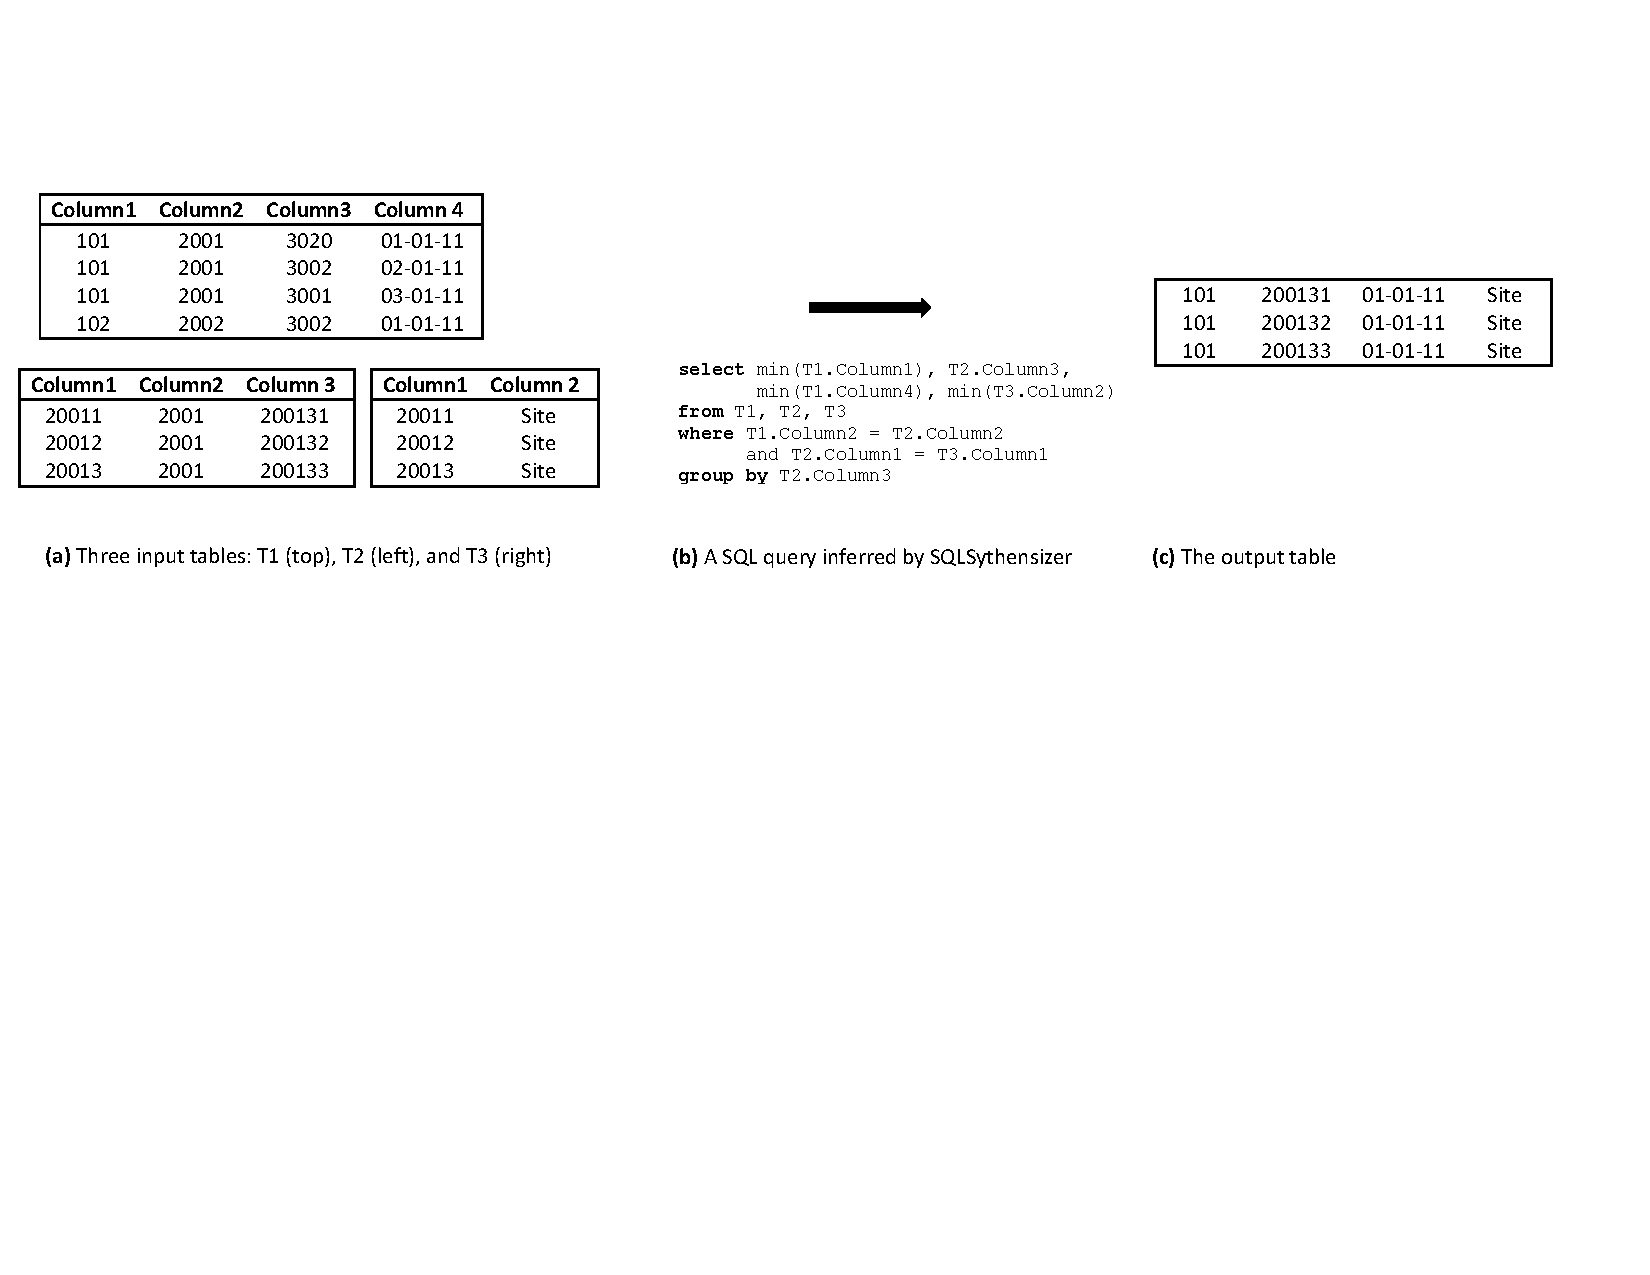
\includegraphics[scale=0.70]{example2}
  \vspace*{-1.0ex}\caption {{\label{fig:example2} Input-output
  examples ((a) and (c)) taken from an online SQL help forum
  thread. \ourtool automatically sythensizes 6 SQL queries that
  can produce the output table from the three input tables.
  (b) shows the highest ranked SQL query.
}}
\end{figure*}

We use a real SQL question from
an online forum\footnote{\url{http://forums.tutorialized.com/sql-basics-113/join-problem-147856.html}} to illustrate
\ourtool's effectiveness.
The question was started by a novice user, who needed help to write a
SQL query to get result from three input tables. In this question, the
novice user described his required query in a few paragraphs of
English, but also include several small, representative input-output
examples as shown in Figure~\ref{fig:example2}, to better express
his intention. 
This question receives no replies as of April 2013 and we speculated that
writing a SQL query to join three tables to produce certain output results
is non-trivial.

We ran \ourtool on the input-output examples
in Figure~\ref{fig:example2}. The tool produced 6 valid answers
in less than 1 minutes, all of which satisfy the given examples. The
highest ranked SQL query is shown in Figure~\ref{fig:example2},
which is quite unintuitive to write. The SQL query in
Figure~\ref{fig:example2}
first joins three input tables
on columns \CodeIn{T1.Column2}, \CodeIn{T2.Column2},
\CodeIn{T2.Column1}, and \CodeIn{T3.Column1} using some
selected columns, and then aggregates the results based on
column \CodeIn{Table2.Column3}'s value. Finally, it
returns the minimal values of columns \CodeIn{T1.Column1}, \CodeIn{T1.Column4}, and \CodeIn{T3.Column2}
from each aggregated group as the results.




\subsubsection{Performance}

We measured \ourtool�s performance by recording the average
time cost in producing a ranked list of SQL queries. 
As shown in Figure~\ref{}, the performance of \ourtool is
reasonable. On average, it uses less than XX minutes to
produce the results in one interative round.
Most of the time is spent querying the backend
database to validate the correctness of each sythesized SQL query.
\todo{caching might be helpful}



\subsubsection{Number of Interactive Rounds}
This is a measure of the generalization power of
the conditional learning part of the algorithm and
the ranking scheme. We observed that the tool typically requires
just \todo{XXX} round of interaction, when the user is smart
enough to give an example for each input format (which
typically range from 1 to
3) to start with. This was indeed the case
for most scenarios in our benchmarks, even though our algorithm
can function robustly without this assumption. The maximum number
of interactive rounds required in any scenario was \todo{XXX}
(with 2 to 3 being a more typical number). \todo{the largest table}
The maximum number of examples
required in any scenario over all possible interactions was 10.

\subsubsection{Comparison with a Previous Technique}.
\todo{not ready yet}

\subsection{Initial Experience}

We deployed the beta-test version of \ourtool
to a small number of developers and have been
using it ourselves, and refining it, since
early May 2012. Designing and deploying \ourtool, along with
feedback from the handful of users, has helped
us to better understand the issues and to improve
the tool's design.

Here is one example piece of feedback from an
external user, via private communication:

\todo{some quote from users}

Prior to developing \ourtool, we studied
over 100 forum posts about common problems
about writing correct SQL queries.
\todo{most of them use examples}
We anticipate that future user studies will
identify additional strengths and weaknesses that will allow us to
further improve \ourtool.




\subsection{Experimental Discussion}

\noindent \textbf{\textit{Limitations.}}
The experiments indicate several limitations
of our technique. First, XXX Second, XXX..
\todo{fill above}

\vspace{1mm}
\noindent \textbf{\textit{Threats to Validity.}}
There are three major threats to validity
in our evaluation. First, the \exnum textbook exercises
and \pnum forum problems may not be representative. Thus,
we can not claim the results can be generalized to an
arbitrary scenario. Second, we only compared
\ourtool with \todo{comparison results}. Using
other query inference and recommendation techniques~\cite{}
might achieve different results. Third, \todo{about user study}


\vspace{1mm}
\noindent \textbf{\textit{Experimental Conclusions.}}
We have three chief findings: \textbf{(1)}
The supported SQL subset in \ourtool is
expressive enough to describe a variety of database queries.
\textbf{(2)} \ourtool efficiently synthesizes desirable SQL
queries on \todo{how many} for both textbook exercises
and online forum problems, with a small amount of human
effort small input-output examples.
\textbf{(3)} \ourtool infers more SQL queries
than existing techniques~\cite{}. \todo{edit}




